% -*- TeX -*- -*- UK -*-
% ----------------------------------------------------------------
% arXiv Paper ************************************************
%
% Subhaneil Lahiri's template
%
% Before submitting:
%    Comment out hyperref
%    Comment out showkeys
%    Replace \newcommand{\mlim}[2]{{\stackrel{\scriptstyle #1}{#2}}}
\newcommand{\ra}{\rightarrow}
\newcommand{\lr}{\leftrightarrow}
\newcommand{\cdt}{\!\cdot\!}
\newcommand{\vp}{\vspace{0.5cm}}
\newcommand{\degs}{^\circ}
%
%e.g., i.e. with normal spaces
\newcommand{\eg}{e.g.\ }
\newcommand{\ie}{i.e.\ }
\newcommand{\cf}{cf.\ }
\newcommand{\etc}{etc.\ }
%
% indices
\newcommand{\up}[1]{\mbox{}^{#1}}
\newcommand{\dn}[1]{\mbox{}_{#1}}
\newcommand{\rp}[1]{^{(#1)}}
\newcommand{\lp}[1]{_{(#1)}}
%
% brackets etc.
\newcommand{\prn}[1]{\left ( #1 \right )}
\newcommand{\brc}[1]{\left\{ #1 \right\}}
\newcommand{\brk}[1]{\left [ #1 \right ]}
\newcommand{\abs}[1]{\left\lvert #1 \right\rvert}
\newcommand{\nrm}[1]{\left\lVert #1 \right\rVert}
\newcommand{\av}[1]{\left\langle #1 \right\rangle}
%
% QM Dirac notation
\newcommand{\bra}[1]{\left\langle #1 \right \rvert}
\newcommand{\ket}[1]{\left \lvert #1 \right\rangle}
\newcommand{\braket}[2]{\left\langle #1 \midddle | #2 \right\rangle}
\newcommand{\bracket}[3]{\left\langle #1 \middle | #2 \middle | #3 \right\rangle}
%
% Derivatives, etc. First argument is optional.
\newcommand{\diff}[3][\rule{0mm}{0mm}]{\frac{\mathrm{d}^{#1} #2}{\mathrm{d}{#3}^{#1}}}
\newcommand{\pdiff}[3][\rule{0mm}{0mm}]{\frac{\partial^{#1} #2}{\partial {#3}^{#1}}}
\newcommand{\pdiffc}[3][\rule{0mm}{0mm}]{\left (\frac{\partial #2}{\partial {#3}}\right )_{\!\!#1}}
\newcommand{\pdl}[1][\rule{0mm}{0mm}]{\overleftarrow{\partial}_{#1}}
\newcommand{\pdr}[1][\rule{0mm}{0mm}]{\overrightarrow{\partial}_{#1}}
\newcommand{\pdlr}[1][\rule{0mm}{0mm}]{\overleftrightarrow{\partial_{#1}}}
\newcommand{\fdf}[2]{\frac{\delta #1}{\delta #2}}
\newcommand{\intd}[1]{\int\!\dr #1\,}
%
% Un-italicised letters
\newcommand{\dr}{\mathrm{d}}
\newcommand{\e}{\mathrm{e}}
\newcommand{\ir}{\mathrm{i}}
\DeclareMathOperator{\tr}{tr}
\DeclareMathOperator{\Tr}{Tr}
\DeclareMathOperator{\Det}{Det}
%
% The default \Im and \Re look crap
\renewcommand{\Im}{\operatorname{\mathfrak{Im}}}
\renewcommand{\Re}{\operatorname{\mathfrak{Re}}}
%
% Referencing sections, figures, etc
\newcommand{\sref}[1]{\S\ref{#1}}
\newcommand{\cref}[1]{Ch.\ref{#1}}
\newcommand{\Cref}[1]{Ch.\ref{#1}}
\newcommand{\fref}[1]{fig.\ref{#1}}
\newcommand{\Fref}[1]{Fig.\ref{#1}}
\newcommand{\tref}[1]{tab.\ref{#1}}
\newcommand{\Tref}[1]{Tab.\ref{#1}}
%
\newcommand{\nn}{\nonumber}
%
% Put the preprint numbers in the top right corner of the page.
% Use after \maketitle.
% First argument: How high it needs to be raised,
% Second argument: Width of the box,
% Third argument: The preprint numbers.
\newcommand{\preprintno}[3]{\hfill\raisebox{#1}[0cm][0cm]{
\begin{minipage}[t]{#2}\begin{flushright} #3 \end{flushright}\end{minipage}}
\vspace*{-\baselinestretch\baselineskip}}
%
% If you have changed the line spacing, e.g. with \renewcommand{\baselinestretch}{1.5},
% the command \sgap produces a line break with the normal spacing.
\newlength{\lingap}
\setlength{\lingap}{\baselinestretch\baselineskip}
\addtolength{\lingap}{-\baselineskip}
\newcommand{\sgap}{\\[-\lingap]}
 with its contents
%       or include mydefs.tex in zip/tar file
%    Replace %
\newcommand{\CD}{\mathcal{D}}
\newcommand{\CE}{\mathcal{E}}
\newcommand{\CG}{\mathcal{G}}
\newcommand{\CH}{\mathcal{H}}
\newcommand{\CK}{\mathcal{K}}
\newcommand{\CO}{\mathcal{O}}
\newcommand{\CL}{\mathcal{L}}
\newcommand{\CM}{\mathcal{M}}
\newcommand{\CN}{\mathcal{N}}
\newcommand{\CV}{\mathcal{V}}
\newcommand{\CZ}{\mathcal{Z}}
%
\newcommand{\dM}{\mathfrak{M}}
\newcommand{\dmd}{\mathfrak{d}}
\newcommand{\dmD}{\mathfrak{D}}
%
\newcommand{\R}{\mathbb{R}}
\newcommand{\C}{\mathbb{C}}
\newcommand{\CP}{\mathbb{CP}}
\newcommand{\Z}{\mathbb{Z}}
%
\newcommand{\ad}{{\dot{\alpha}}}
\newcommand{\bd}{{\dot{\beta}}}
\newcommand{\gd}{{\dot{\gamma}}}
\newcommand{\dd}{{\dot{\delta}}}
\newcommand{\ed}{{\dot{\epsilon}}}
%
\newcommand{\bs}{\overline{\sigma}}
\newcommand{\br}{\overline{\rho}}
\newcommand{\bpsi}{\overline{\psi}}
\newcommand{\bchi}{\overline{\chi}}
\newcommand{\bPsi}{\overline{\Psi}}
\newcommand{\bQ}{\overline{Q}}
\newcommand{\bS}{\overline{S}}
\newcommand{\bJ}{\overline{J}}
\newcommand{\zb}{{\bar z}}
\newcommand{\wb}{{\overline w}}
\newcommand{\cb}{{\bar c}}
\newcommand{\ab}{{\bar a}}
\newcommand{\bb}{{\bar b}}
\newcommand{\bp}{{\bar\partial}}
%
\newcommand{\p}{\partial}
\newcommand{\apm}{{\alpha^{\prime}}}
\newcommand{\adg}{a^\dagger}
\newcommand{\psq}{^{\prime\,2}}
\newcommand{\ppsq}{^{\prime\prime\,2}}
\newcommand{\half}{\frac{1}{2}}
%
 with its contents
%       or include newsymb.tex in zip/tar file
%    Put this file, the .bbl file, any picture or
%       other additional files and natbib.sty
%       file in a zip/tar file
%
% **** -----------------------------------------------------------
\documentclass[12pt]{article}
%
% Preamble:
\usepackage{a4wide}
\input{sl_preamble.tex}
\input{sl_graphics_preamble.tex}
\graphicspath{{figs/}}
%
% >> Only for drafts! <<
\usepackage[notref,notcite]{showkeys}
%
% ----------------------------------------------------------------
%\numberwithin{equation}{section}
%\renewcommand{\baselinestretch}{1.5}
% ----------------------------------------------------------------
% New commands etc.
\input{sl_definitions.tex}
\input{sl_symbols.tex}
%matrices
\newcommand{\inv}{^{-1}}
\newcommand{\dg}{^\dagger}
\newcommand{\trans}{^\mathrm{T}}
\newcommand{\I}{\mathbf{I}}
\newcommand{\omb}{\overline{\omega}}
\newcommand{\bt}{\overline{\tau}}
\newcommand{\dw}{\dr w}
\newcommand{\dwb}{\dr\overline{w}}
\newcommand{\du}{\dr u}
\newcommand{\dub}{\dr\bar{u}}
\newcommand{\dv}{\dr v}
\newcommand{\dvb}{\dr\bar{v}}
\newcommand{\opo}{\prn{1+\abs{\omega}^2}}
\newcommand{\omo}{\prn{1-\abs{\omega}^2}}
% ----------------------------------------------------------------
%
%%%%%%%%%%%%%%%%%%%%%%%%%%%%%%%%%%%%%%%%%%%%%%%%%%%%%%%%%%%%%%%%%%%%%%%%%%
% Title info:
\title{Illusions of criticality in high-dimensional autoregressive models}
%
% Author List:
%
\author{Subhaneil Lahiri and Surya Ganguli
%
}

\begin{document}

\maketitle


%%%%%%%%%%%%%%%%%%%%%%%%%%%%%%%%%%%%%%%%%%%%%%%%%%%%%%%%%%%%%%%%%%%%%%%%%%


\begin{abstract}
  We look at the eigenvalue spectrum of high-dimensional autoregressive models when applied to white-noise.
\end{abstract}

\tableofcontents

%%%%%%%%%%%%%%%%%%%%%%%%%%%%%%%%%%%%%%%%%%%%%%%%%%%%%%%%%%%%%%%%%%%%%%%%%%
% Beginning of Article:
%%%%%%%%%%%%%%%%%%%%%%%%%%%%%%%%%%%%%%%%%%%%%%%%%%%%%%%%%%%%%%%%%%%%%%%%%%

\section{The problem}\label{sec:theprob}

Consider a model of the following type
%
\begin{equation}\label{eq:model}
  x(t+1) = A x(t) + \text{noise},
\end{equation}
%
where $x(t)$ is an $N$-element vector and $A$ is an $N\times N$ matrix.

Suppose we have a sample of $P$ consecutive times, so $x$ is an $N\times P$ matrix.
We can perform a least-squares estimate of $A$ by minimising the quantity
%
\begin{equation}\label{eq:minL}
  \half\sum_{i,\mu} \prn{ x_{i\mu+1} - \sum_j A_{ij} x_{j\mu} }^2 = \half\Tr \prn{xU-Ax}\prn{xU-Ax}\trans,
\end{equation}
%
where $U$ is a shift matrix.
It will be useful to use periodic boundary conditions in time, \ie $x_{iP+1}\sim x_{i1}$,
as this will make $U$ orthogonal:
%
\begin{equation}\label{eq:Udef}
  U_{\mu\nu} = \delta_{\mu\nu+1} + \delta_{\mu1}\delta_{\nu P}.
\end{equation}
%
The estimate of $A$ is then
%
\begin{equation}\label{eq:Aest}
  A = \prn{xUx\trans}\prn{xx\trans}\inv.
\end{equation}
%

Suppose we attempted this analysis in a situation where there really is no structure,
\ie when $x(t)$ is white noise.
Then the true optimal $A$ would be 0.
However, with finite $P$ the estimate \eqref{eq:Aest} will not be zero.

We will look at the average eigenvalue distribution:
%
\begin{equation}\label{eq:eigdist}
  \rho(\omega) = \av{\rho_A(\omega)}_x,
  \qquad
  \rho_A = \sum_{i=1}^N \delta(\omega-\lambda_i),
\end{equation}
%
where $\lambda_i$ are the eigenvalues of $A$ in \eqref{eq:Aest} and
the components of $x$ are iid gaussian random variables with mean 0 and variance 1.
This quantity is most relevant in the limit of large $N$ and $P$.
We will keep the quantity $\alpha=P/N$ fixed in this limit.

Following \cite{Sommers1988asymmetric}, this can be computed from a potential:
%
\begin{equation}\label{eq:potential}
  \rho_A(\omega) = -\nabla^2 \Phi_A(\omega),
  \qquad
  \Phi_A(\omega) = -\frac{1}{4\pi N} \ln\det \brk{(\omb-A\trans)(\omega-A)}.
\end{equation}
%
We define a partition function
%
\begin{equation}\label{eq:partfn}
  \Phi_A(\omega) = \frac{1}{4\pi N} \ln Z_A(\omega),
  \qquad
  Z_A(\omega) = \det \brk{(\omb-A\trans)(\omega-A)}\inv.
\end{equation}
%
The problem is now to compute $\av{\ln Z_A(\omega)}_x$.


\section{The solution}\label{sec:solution}

In \sref{sec:simplederiv} we will present a simplified derivation and in \sref{sec:replicader} we will fill in the gaps and justify the assumptions used in \sref{sec:replicader}.
The result will be:
%
%\begin{equation}\label{eq:phisol}
%\begin{aligned}
\begin{align}
\label{eq:rssol}
  rs &= \frac{\alpha^2 \brk{ -(\alpha-1)\opo \pm \sqrt{ (\alpha-1)^2\opo^2 + (2\alpha-1)\omo^2 } }}{(\alpha-1)\omo^2},\\
\label{eq:zmsol}
  \zeta_- &= \frac{1+\abs{\omega}^2}{2\omb} - \frac{\alpha^2}{2(\alpha-1)\omb rs},\\
\label{eq:phisol}
  \Phi(\omega) &= \frac{1}{4\pi}\max_\pm\brk{ (1-\alpha)\ln(rs) -\alpha\ln\prn{\abs{\frac{\omega}{\zeta_-}}} -\ir\alpha\arg(-\omega)},
\end{align}
%\end{aligned}
%\end{equation}
%
subject to the restriction
%
\begin{align}%\label{eq:phisolreq}
%\label{eq:rsreq}
%  rs &\leq \frac{\alpha^2(2\alpha^3-2\alpha+1)}{2(\alpha+1)(\alpha-1)^3\opo}.
%  \\
\label{eq:zmreq}
  \abs{\zeta_-} &\leq 1,
\end{align}
%
The imaginary part of $\Phi$ is harmonic, and will therefore not contribute to the density \eqref{eq:potential}.
This means that everything has a rotation symmetry.

Can we have a crossover between the two choices in \eqref{eq:rssol} as $\omega$ varies?
This would require a point where the two solutions are equal:
%
\begin{equation}\label{eq:rsdegenerate}
\begin{aligned}
  (\alpha-1)^2\opo^2 + (2\alpha-1)\omo^2 &=0, \\
  \implies \abs{\omega}^2 &= \frac{-(\alpha^2-4\alpha+2) \pm (\alpha-1)\sqrt{1-2\alpha}}{\alpha^2}.
\end{aligned}
\end{equation}
%
This is only possible at $\alpha=1$.

Let's look at two interesting limits. 

First, $\alpha\to1$:
%
\begin{equation}\label{eq:rszmato1}
\begin{aligned}
  rs &\to \pm\frac{1}{(\alpha-1)\omo},\\
  \implies\zeta_- &\to \frac{\opo\mp\omo}{2\omb} =  \quad\omega \quad\text{or}\quad \frac{1}{\omb},
\end{aligned}
\end{equation}
%
with the first choice satisfying \eqref{eq:zmreq} for $\abs{\omega}<1$ and the other for $\abs{\omega}>1$,
%
\begin{equation}\label{eq:phiato1}
  \implies\Phi \to 
  \begin{cases}
    0 &\text{for } \abs{\omega}<1,\\
    -\frac{\ln\abs{\omega}}{2\pi} &\text{for } \abs{\omega}>1.\\
  \end{cases}
\end{equation}
%
This is harmonic everywhere except $\abs{\omega}=1$.
Applying Gauss' law to a circular loop of radius greater than 1, centred at the origin, tells us that the total charge enclosed is 1.
Therefore:
%
\begin{equation}\label{eq:rhoato1}
  \rho(\omega) \to \frac{\delta(\abs{\omega}-1)}{2\pi}
  \quad\text{as}\quad \alpha\to1.
\end{equation}
%


Now, $\alpha\to\infty$:
%
\begin{multline}\label{eq:rsatoinfty}
  rs = -\frac{2\alpha^2\opo}{\omo^2} + \CO(\alpha)
  \quad\text{or}\quad \\
  \frac{\alpha}{1+\abs{\omega}^2} \brk{1 + \frac{1+4\abs{\omega}^2+\abs{\omega}^4}{\alpha\opo^2}
       + \frac{1+6\abs{\omega}^2+18\abs{\omega}^4+6\abs{\omega}^6+\abs{\omega}^8}{\alpha^2\opo^4}
       + \CO(\alpha^{-3})},
\end{multline}
%
which leads to
%
\begin{equation}\label{eq:zmatoinfty}
  \zeta_- = \frac{1+\abs{\omega}^2}{2\omb}
  \quad\text{or}\quad 
  \frac{\omega}{\alpha\opo} \brk{1 + \frac{2\abs{\omega}^2}{\alpha\opo^2} + \CO(\alpha^{-2})},
\end{equation}
%
only the second of which satisfies \eqref{eq:zmreq}. With this choice for both \eqref{eq:rsatoinfty} and \eqref{eq:zmatoinfty}:
%
\begin{equation}\label{eq:phiatoinfty}
  \Phi = -\frac{\ln\opo}{4\pi} + \CO(\alpha^{-1}),
\end{equation}
%
in which we have dropped (infinite) constants.
This results in
%
\begin{equation}\label{eq:rhoatoinfty}
  \rho(\omega) \to \frac{1}{\pi\opo^2}
  \quad\text{as}\quad
  \alpha\to\infty.
\end{equation}
%
This should be a delta function at zero.



\section{Simplified derivation}\label{sec:simplederiv}

In this section, we will present a simplified version of the derivation.
We will make the following simplifying assumption.

At some point, we will treat $x$ as annealed, rather than quenched, disorder:
%
\begin{equation}\label{eq:annealed}
  \av{\ln (\cdots)}_x = \ln\av{\cdots}_x.
\end{equation}
%
We will justify this assumption in \sref{sec:replicader} using the replica trick.
We will see that, with a replica symmetric ansatz, the saddle point has zero off-diagonal replica overlaps.
This means that there is no coupling between the replicas, which produces identical results to the annealed calculation.

We start with the representation of the determinant in \eqref{eq:compgausint}.
However, the matrix in \eqref{eq:partfn} is not positive-definite when $\omb$ is equal to one of the eigenvalues.
We can fix this by adding $\epsilon^2I$ and letting $\epsilon\to0$ at the end.
%
\begin{equation}\label{eq:partfnintz}
\begin{aligned}
  Z_A(\omega) &= \int \prod_i\frac{\dz_i\dzb_i}{2\pi} \exp\prn{
    -z\dg (\omb-A\trans)(\omega-A) z - \epsilon^2 z\dg z} .%\\
%    &=  \int \prod_i\frac{\dz_i\dzb_i}{2\pi} \exp\prn{
%    -z\dg (xx\trans)\inv x(\omb-U)x\trans x(\omega-U)x\trans (xx\trans)\inv z
%    - \epsilon^2 z\dg z}. \\
\end{aligned}
\end{equation}
%
Looking at the expression \eqref{eq:Aest} for $A$, we make the change of variables $z=(xx\trans)w/P$.
%
\begin{equation}\label{eq:partfnintw}
\begin{aligned}
  Z_A(\omega) &= \det(xx\trans)^2 \int \prod_i\frac{\dw_i\dwb_i}{2\pi}\e^{-F/P^2}
    \\
  F &=
     w\dg x(\omb-U\dg)x\trans x(\omega-U)x\trans w + \epsilon^2 w\dg xx\trans xx\trans w .%\\
\end{aligned}
\end{equation}
%
We now take advantage of \eqref{eq:compgausslin} by introducing two standard complex Gaussian random vectors ($C=I$ in \eqref{eq:compgaussnorm}), $u$ and $v$:
%
\begin{equation}\label{eq:partfnintwuv}
\begin{aligned}
  Z_A(\omega) &= \det(xx\trans)^2 \int \prod_i\frac{\dw_i\dwb_i}{2\pi} \av{\e^{\ir F'/P}}_{u,v},\\
  F' &=
    w\dg x(\omb-U\dg)x\trans u + u\dg x(\omega-U)x\trans w + \epsilon w\dg xx\trans v + \epsilon v\dg xx\trans w .%\\
\end{aligned}
\end{equation}
%

Over most of the integration domain, we expect the real inner products ($w\dg w$,$u\dg u$,\ldots) will be $\CO(N)$, whereas the complex inner products ($w\dg u$,$w\trans w$,\ldots) will be $\CO(\sqrt{N})$.
We define some new variables, $\rho,\sigma \text{ and } \tau$, which are zero mean Gaussian random vectors:
%
\begin{equation}\label{eq:rstdef}
\begin{aligned}
  \rho &= x\trans w ,
    & \av{\br_\mu \rho_\nu}_x &= Nr\delta_{\mu\nu} ,
    & r&=\frac{w\dg w}{N}, \\
  \sigma &= x\trans u ,
    & \av{\bs_\mu \sigma_\nu}_x &= Ns\delta_{\mu\nu} ,
    & s&=\frac{u\dg u}{N}, \\
  \tau &= x\trans v,
    & \av{\bt_\mu \tau_\nu}_x &= Nt\delta_{\mu\nu},
    & t&=\frac{v\dg v}{N}, \\
\end{aligned}
\end{equation}
%
with all other covariances negligible in the large $N$ limit.
We can now write
%
\begin{equation}\label{eq:potwuv}
\begin{aligned}
  \av{\ln Z_A(\omega)}_x =&\,  2\av{\ln\det(xx\trans)}_x
  \\&+
          \av{\ln\int \prod_i\brk{ \frac{\dw_i\dwb_i}{2\pi} \frac{\du_i\dub_i}{2\pi} \frac{\dv_i\dvb_i}{2\pi} } \e^{-N(s+t)-\xi\dg A \xi} }_{x} ,
  \\ \text{where}\quad
  \xi =&\, \begin{pmatrix}
           \rho \\
           \sigma \\
           \tau \\
         \end{pmatrix},
 \\
  A =&\, -\frac{\ir}{P}
       \begin{pmatrix}
         0        & \omb-U\dg & \epsilon \\
         \omega-U & 0            & 0 \\
         \epsilon & 0            & 0 \\
       \end{pmatrix},\\
  \av{\xi\xi\dg}_x &=  C = N\begin{pmatrix}
         r & 0 & 0 \\
         0 & s & 0 \\
         0 & 0 & t \\
       \end{pmatrix}.
\end{aligned}
\end{equation}
%
As we only care about the part of $\Phi$ that depends on $\omega$, we can ignore the first term.
We will simplify the second term using \eqref{eq:annealed}, \eqref{eq:compgaussquad} and the relation
%
\begin{equation}\label{eq:spherical}
  \int \prod_i\brk{ \frac{\dw_i\dwb_i}{2\pi} } f(r) = \frac{N^N}{\Gamma(N)} \intd{r} r^{N-1} f(r),
\end{equation}
%
along with similar ones for $u$ and $v$, to get
%
\begin{equation}\label{eq:phiintsimple}
\begin{aligned}
  \Phi(\omega) &= \text{const.} + \frac{1}{4\pi N} \ln \int \frac{\dr r}{r} \frac{\dr s}{s} \frac{\dr t}{t}
      (rst)^N\e^{-N(s+t)} \av{\e^{-\xi\dg A \xi}}_x\\
      &= \text{const.} + \frac{1}{4\pi N} \ln \int \frac{\dr r}{r} \frac{\dr s}{s} \frac{\dr t}{t}
      \,\frac{\exp[N(\ln(rst)-s-t)]}{\det(I+CA)}.
\end{aligned}
\end{equation}
%

As $U$ is unitary, all the blocks in these matrices commute.
Therefore, we can evaluate the determinant with some help from \cite{silvester2000determinants}.
Also noting that the eigenvalues of $U$ are $\exp(2\pi\ir k/P)$, with $k\in\Z_P$:
%
\begin{equation}\label{eq:detsimple}
\begin{aligned}
  \ln\det(I+CA) &= \ln\det\brk{\frac{1}{\alpha^3}
       \begin{pmatrix}
         \alpha           & -\ir r(\omb-U\dg) & -\ir\epsilon r \\
         -\ir s(\omega-U) & \alpha               & 0 \\
         -\ir\epsilon t   & 0                    & \alpha \\
       \end{pmatrix}}\\
     &= \ln\det\brk{\frac{\alpha^2+\epsilon^2rt + rs(\omb-U\dg)(\omega-U)}{\alpha^2}}\\
     &= \sum_{k=0}^{P-1} \ln\brk{ \frac{\alpha^2+\epsilon^2rt + rs (\omb-\e^{-2\pi\ir k/P}) (\omega-\e^{2\pi\ir k/P})} {\alpha^2}}\\
     &= \frac{P}{2\pi} \intd[_0^{2\pi}]{\phi} \ln\brk{ \frac{\alpha^2+\epsilon^2rt + rs (\omb-\e^{-\ir\phi}) (\omega-\e^{\ir\phi})} {\alpha^2}}\\
     &= \frac{P}{2\pi\ir} \int \frac{\dr\zeta}{\zeta} \, \ln \brk{\frac{G(\zeta)}{\alpha^2\zeta}},
\end{aligned}
\end{equation}
%
$(C\inv+A)$ IS NON-NORMAL!
where the function $G(\zeta)$ is defined in \sref{sec:Gamma}, in particular \eqref{eq:Gammadef}.
The denominator of the logarithm contributes a factor that is independent of $\omega$, which can be safely ignored.

If we factorise $G(\zeta)$, we get some contour integrals of the form discussed in \sref{sec:contourints}, the result of which appears in \eqref{eq:countourintresult}.
From \eqref{eq:zpzm}, we know that only one of the zeros of $G(\zeta)$ will ie inside the contour.
We find that
%
\begin{equation}\label{eq:detsimpleresult}
\begin{aligned}
  \ln\det(I+CA) &= \text{const.} + P[\ln(-rs\omb) + \ln\zeta_+ + \ln\zeta_- - \ln(\min\abs{\zeta_\pm})]   \\
   &= \text{const.} + P\ln\prn{-\frac{rs\omega}{\min\abs{\zeta_\pm}}}.
\end{aligned}
\end{equation}
%

Now, if we use the saddle-point approximation of the integrals over $r$, $s$ and $t$ in \eqref{eq:phiintsimple}, which becomes exact in the limit of large $N$ and $P$, we find
%
\begin{equation}\label{eq:phisaddlesimple}
  \Phi(\omega) = \frac{1}{4\pi} \max_{r,s,t} \brk{ \ln(rst) - s - t -\alpha\ln\prn{-\frac{rs\omega}{\min\abs{\zeta_\pm}}}}.
\end{equation}
%
One can show that (see \sref{sec:replicader}, in particular \eqref{eq:repsaddlesol} and \eqref{eq:rOe}) the maximum has
%
\begin{equation}\label{eq:saddleOe}
  r \sim \CO(\epsilon\inv),
  \qquad
  s \sim \CO(\epsilon),
  \qquad
  t \sim \CO(1),
  \qquad
  rs \sim \CO(1).
\end{equation}
%
If we take $\epsilon\to0$, we find that $\Phi$ depends on $r$, $s$ and $t$ in the combinations $rs$ and $t$:
%
\begin{equation}\label{eq:phimaxsimple}
\begin{aligned}
  \Phi(\omega) &= \frac{1}{4\pi} \max_{rs,t} \brk{ (1-\alpha)\ln(rs)+\ln t - t -\alpha\ln\prn{-\frac{\omega}{\min\abs{\zeta_\pm}}}}\\
  \pdiff{\Phi}{(rs)} &= \frac{1-\alpha}{rs} + \alpha\Re\prn{\frac{\alpha^2}{rs G'(\min\abs{\zeta_\pm})}} ,\\
  \pdiff{\Phi}{t}&= \frac{1}{t} - 1 .
\end{aligned}
\end{equation}
%
Setting these derivatives to zero requires
%
\begin{equation}\label{eq:saddlereq}
  \abs{\zeta_-}\leq1,
\end{equation}
%
in which case
%
\begin{equation}\label{eq:saddlesol}
\begin{aligned}
  t &=1, \\
  rs &= \frac{\alpha^2 \brk{ -(\alpha-1)\opo \pm \sqrt{ (\alpha-1)^2\opo^2 + (2\alpha-1)\omo^2 } }}{(\alpha-1)\omo^2},\\
  \zeta_- &= \frac{1+\abs{\omega}^2}{2\omb} - \frac{\alpha^2}{2(\alpha-1)\omb rs},\\
 \Phi(\omega) &= \frac{1}{4\pi}\max_\pm\brk{ (1-\alpha)\ln(rs) -\alpha\ln\prn{-\frac{\omega}{\abs{\zeta_-}}}}.
\end{aligned}
\end{equation}
%






\section{Full, replica-tastic derivation}\label{sec:replicader}


The starting point for this version of the derivation will be \eqref{eq:partfnintwuv} and \eqref{eq:potwuv}:
%
\begin{equation}\label{eq:phiint}
  \begin{aligned}
    \Phi(\omega) &= \text{const.} + \frac{1}{4\pi N} \av{\ln \widetilde{Z}}_x, \\
    \widetilde{Z} &= \int \prod_i\brk{ \frac{\dw_i\dwb_i}{2\pi} \frac{\du_i\dub_i}{2\pi} \frac{\dv_i\dvb_i}{2\pi} } \e^{-F''}, \\
    F'' &=  u\dg u + v\dg v -\frac{\ir}{P}\brk{ w\dg x(\omb-U\dg)x\trans u + \epsilon w\dg xx\trans v + \text{c.c.} }.
  \end{aligned}
\end{equation}
%
We will use the replica trick., \ie we rewrite the logarithm as
%
\begin{equation}\label{eq:replicatrick}
  \ln \widetilde{Z} = \left. \pdiff{( \widetilde{Z}^n )}{n}\right\rvert_{n=0}.
\end{equation}
%
For integer $n$, we can compute $\widetilde{Z}^n$ by creating $n$ replicas of the system,
We then let $n\to0$ after averaging over $x$.
We index these replicas with $a,b=1,\ldots,n$:
%
\begin{equation}\label{eq:phirep}
    \begin{aligned}
    \Phi(\omega) &= \frac{1}{4\pi N}  \left.\pdiff{}{n}\av{
       \int \prod_{ia}\brk{ \frac{\dw_{ia}\dwb_{ia}}{2\pi} \frac{\du_{ia}\dub_{ia}}{2\pi} \frac{\dv_{ia}\dvb_{ia}}{2\pi} } \e^{-F'''}
       }_x\right\rvert_{n=0}, \\
    F''' &= \sum_a  u_a\dg u_a + v_a\dg v_a -\frac{\ir}{P}\brk{ w_a\dg x(\omb-U\dg)x\trans u_a + \epsilon w_a\dg xx\trans v_a + \text{c.c.} }.
  \end{aligned}
\end{equation}
%

Over most of the integration domain, we expect the Hermitian overlaps ($w_a\dg w_b, u_a\dg u_b,\ldots$) will be $\CO(N)$, whereas the non-Hermitian overlaps ($w_a\dg u_b, w_a\trans w_b,\ldots$) will be $\CO(\sqrt{N})$.
We define some new variables, $\rho_a,\sigma_a \text{ and } \tau_a$, which are zero mean Gaussian random vectors:
%
\begin{equation}\label{eq:reprstdef}
\begin{aligned}
  \rho_a &= x\trans w_a ,
    & \av{\bar{\rho}_{\mu a} \rho_{\nu b}}_x &= N\delta_{\mu\nu}R_{ab} ,
    & R_{ab}&=\frac{w_a\dg w_b}{N}, \\
  \sigma_a &= x\trans u_a ,
    & \av{\bar{\sigma}_{\mu a} \sigma_{\nu b}}_x &= N\delta_{\mu\nu}S_{ab} ,
    & S_{ab}&=\frac{u_a\dg u_b}{N}, \\
  \tau_a &= x\trans v_a,
    & \av{\bar{\tau}_{\mu a} \tau_{\nu b}}_x &= N\delta_{\mu\nu}T_{ab},
    & T_{ab}&=\frac{v_a\dg v_b}{N}, \\
\end{aligned}
\end{equation}
%
with all other covariances negligible in the large $N$ limit.
%
\begin{equation}\label{eq:phirepxi}
    \begin{aligned}
    \Phi(\omega) &= \frac{1}{4\pi N}  \left.\pdiff{}{n}
       \int \prod_{ia}\brk{ \frac{\dw_{ia}\dwb_{ia}}{2\pi} \frac{\du_{ia}\dub_{ia}}{2\pi} \frac{\dv_{ia}\dvb_{ia}}{2\pi} }
       \av{\e^{-N\Tr(S+T) - \xi\dg A \xi}}_x
       \right\rvert_{n=0}, \\
     &= \frac{1}{4\pi N}  \left.\pdiff{}{n}
       \int \prod_{ia}\brk{ \frac{\dw_{ia}\dwb_{ia}}{2\pi} \frac{\du_{ia}\dub_{ia}}{2\pi} \frac{\dv_{ia}\dvb_{ia}}{2\pi} }
       \e^{-NE(R,S,T)}
       \right\rvert_{n=0},
\end{aligned}
\end{equation}
%
where
%
\begin{equation}\label{eq:overlapenergy}
\begin{aligned}
  E(R,S,T) &= \Tr(S+T) + \frac{1}{N} \ln \det (I+CA),\\
  \xi &= \begin{pmatrix}
           \rho \\
           \sigma \\
           \tau \\
         \end{pmatrix},
 \\
  A &= -\frac{\ir}{P}
       \begin{pmatrix}
         0        & \omb-U\dg & \epsilon \\
         \omega-U & 0            & 0 \\
         \epsilon & 0            & 0 \\
       \end{pmatrix}\otimes I,\\
  \av{\xi\xi\dg}_x &=  C = N I\otimes
       \begin{pmatrix}
         R & 0 & 0 \\
         0 & S & 0 \\
         0 & 0 & T \\
       \end{pmatrix}.  \end{aligned}
\end{equation}
%

It will be helpful to separate the integrals over $w,u\text{ and }v$ into an integral over values of $w,u\text{ and }v$ with the same overlap and an integral over values of the overlap.
This can be done by inserting factors like the following into the integral:
%
\begin{equation}\label{eq:overlapdelta}
  \int \dr R_{ab} N^{n^2} \delta (N R_{ab} - w_a\dg w_b ) = 1.
\end{equation}
%
We define
%
\begin{equation}\label{eq:overlapentropy}
  S(R) = \frac{1}{N} \int \prod_{ia}\brk{ \frac{\dw_{ia}\dwb_{ia}}{2\pi} }
  N^{n^2} \delta (N R_{ab} - w_a\dg w_b )
   = \ln\det R + \text{const.}
\end{equation}
%
with the final expression valid in the large $N$ limit.
Then \eqref{eq:phirepxi} reduces to
%
\begin{equation}\label{eq:phioverlap}
  \Phi(\omega) = \frac{1}{4\pi N}  \left.\pdiff{}{n}
       \int \dr R_{ab} \dr S_{ab} \dr T_{ab}
       \,\e^{-N(E(R,S,T)-S(R)-S(S)-S(T))}
       \right\rvert_{n=0}.
\end{equation}
%
We will perform this integral in the large $N$ limit with the saddle point method.

We make the following, replica-symmetric ans\"atze for the saddle-point:
%
\begin{equation}\label{eq:RSansatze}
  R_{ab} = r_0\delta_{ab} + r_1,
  \qquad
  S_{ab} = s_0\delta_{ab} + s_1,
  \qquad
  T_{ab} = t_0\delta_{ab} + t_1.
\end{equation}
%
A matrix of this form has $(n-1)$ eigenvalues equal to $r_0$ and one eigenvalue equal to $(r_0+nr_1)$.
Therefore,
%
\begin{equation}\label{eq:RSentropy}
  S(R) = \ln\det R = (n-1)\ln r_0 + \ln(r_0 +n r_1) = n\ln r_0 + \frac{nr_1}{r_0} + \CO(n^2).
\end{equation}
%
The replica symmetric form of $R,S<,T$ and the unitarity of $U$ means that all the blocks in \eqref{eq:overlapenergy} commute.
Then, according to \cite{silvester2000determinants},
%
\begin{equation}\label{eq:detrep}
\begin{aligned}
  \ln\det(I+CA) &=  \ln\det\brk{\frac{1}{\alpha^3}
       \begin{pmatrix}
         \alpha                   & -\ir (\omb-U\dg) \otimes R & -\ir\epsilon I\otimes R \\
         -\ir (\omega-U)\otimes S & \alpha                        & 0 \\
         -\ir\epsilon I\otimes T  & 0                             & \alpha \\
       \end{pmatrix}}\\
     &= \ln\det\brk{\frac{\alpha^2+\epsilon^2I\otimes RT + (\omb-U\dg)(\omega-U)\otimes RS}{\alpha^2}}.
\end{aligned}
\end{equation}
%
Note that
%
\begin{equation}\label{eq:overlapprod}
  (RS)_{ab} = r_0s_0 \delta_{ab} + r_0 s_1 + r_1 s_0 + \CO(n),
\end{equation}
%
and similar for $RT$, so these will have a similar eigenvalue structure to $R$, with the same eigenvectors.
Also, the eigenvalues of $U$ are $\exp(2\pi\ir k/P)$, with $k\in\Z_P$.
Therefore:
%
\begin{equation}\label{eq:detrepints}
\begin{aligned}
  \ln\det(I+CA) &=  \sum_{k=0}^{P-1}
    n \left\{
      \ln\brk{ \frac{\alpha^2+\epsilon^2r_0t_0 + r_0s_0 (\omb-\e^{-2\pi\ir k/P}) (\omega-\e^{2\pi\ir k/P})} {\alpha^2}}
    \right.\\
    &\qquad\quad \left.+
      \frac{ \epsilon^2 (r_0t_1+r_1t_0) + (r_0s_1+r_1s_0) (\omb-\e^{-2\pi\ir k/P}) (\omega-\e^{2\pi\ir k/P})} { \alpha^2+\epsilon^2r_0t_0 + r_0s_0 (\omb-\e^{-2\pi\ir k/P}) (\omega-\e^{2\pi\ir k/P})}
    \right\}\\
   &\qquad +\CO(n^2)\\
    &= \frac{nP}{2\pi} \intd[_0^{2\pi}]{\phi} \left\{
     \ln\brk{ \frac{\alpha^2+\epsilon^2r_0t_0 + r_0s_0 (\omb-\e^{-\ir\phi}) (\omega-\e^{\ir\phi})} {\alpha^2}}
    \right.\\
    &\qquad\quad \left.+
      \frac{ \epsilon^2 (r_0t_1+r_1t_0) + (r_0s_1+r_1s_0) (\omb-\e^{-\ir\phi}) (\omega-\e^{\ir\phi})} { \alpha^2+\epsilon^2r_0t_0 + r_0s_0 (\omb-\e^{-\ir\phi}) (\omega-\e^{\ir\phi})}
    \right\}\\
    &= \frac{nP}{2\pi\ir} \int \frac{\dr\zeta}{\zeta} \left\{ \ln \brk{\frac{G(\zeta)}{\alpha^2\zeta}}
    \right.\\
    &\qquad\quad \left.+
      \frac{ \epsilon^2 (r_0t_1+r_1t_0)\zeta + (r_0s_1+r_1s_0) (\omb\zeta-1) (\omega-\zeta)} {G(\zeta)}
    \right\},
\end{aligned}
\end{equation}
%
where the function $G(\zeta)$ is defined in \sref{sec:Gamma}, in particular \eqref{eq:Gammadef}.
The first integral was computed in \eqref{eq:detsimpleresult}.
The second can be computed with the residue theorem.
The integrand has poles at $\zeta\in\brc{0,\zeta_+,\zeta_-}$, with only one of the last two lying inside the contour \eqref{eq:zppzm}.
%
\begin{multline}\label{eq:repcontoutint}
  \frac{1}{2\pi\ir} \int \frac{\dr\zeta}{\zeta}\,
    \frac{ \epsilon^2 (r_0t_1+r_1t_0)\zeta + (r_0s_1+r_1s_0) (\omb\zeta-1) (\omega-\zeta)} {G(\zeta)} \\
    \begin{aligned}
      &= \frac{(r_0s_1+r_1s_0)(-\omega)}{G(0)}
      + \frac{ \epsilon^2 (r_0t_1+r_1t_0)\zeta_\pm + (r_0s_1+r_1s_0) (\omb\zeta_\pm-1) (\omega-\zeta_\pm)} {\zeta_\pm G'(\zeta_\pm)} \\
      &= \frac{r_0s_1+r_1s_0}{r_0s_0}\prn{1-\frac{\alpha^2+\epsilon^2r_0t_0} {G'(\zeta_\pm)}}
      + \frac{ \epsilon^2 (r_0t_1+r_1t_0)} {G'(\zeta_\pm)} .
    \end{aligned}
\end{multline}
%

Combining all of this gives:
%
\begin{equation}\label{eq:phimaxrep}
\begin{aligned}
  \Phi(\omega) =\, \frac{1}{4\pi} \max_{r_{0,1},s_{0,1},t_{0,1}}& \left\{
    \ln(r_0s_0t_0) + \frac{r_1}{r_0} + \frac{s_1}{s_0} + \frac{t_1}{t_0}
    -(s_0 + s_1 + t_0 + t_1)
    \right.\\&\left.
    - \alpha\ln\prn{-\frac{r_0s_0\omega}{\abs{\zeta_\pm}}}
    - \frac{\alpha(r_0s_1+r_1s_0)}{r_0s_0}\prn{1-\frac{\alpha^2+\epsilon^2r_0t_0} {G'(\zeta_\pm)}}
    \right.\\&\left.
    - \frac{ \alpha\epsilon^2 (r_0t_1+r_1t_0)} {G'(\zeta_\pm)}
    \right\}.
\end{aligned}
\end{equation}
%
To find the maximum, we must set to zero the following derivatives
%
\begin{equation}\label{eq:phidiff1}
\begin{aligned}
  \pdiff{(4\pi\Phi)}{r_1} &= \frac{1}{r_0} - \frac{\alpha}{r_0} + \frac{\alpha^3}{r_0G'(\zeta_\pm)},  \\
  \pdiff{(4\pi\Phi)}{s_1} &= \frac{1}{s_0} - 1 - \frac{\alpha}{s_0} + \frac{\alpha(\alpha^2+\epsilon r_0 t_0 )}{s_0G'(\zeta_\pm)},  \\
  \pdiff{(4\pi\Phi)}{t_1} &= \frac{1}{t_0} - 1 - \frac{\alpha\epsilon^2r_0}{G'(\zeta_\pm)}.
\end{aligned}
\end{equation}
%
Solving these equations gives
%
\begin{equation}\label{eq:repsaddlesol}
\begin{aligned}
  s_0 &= \frac{(\alpha-1)\epsilon^2r_0}{\alpha^2}, \qquad
  t_0 &= 1 - s_0,\qquad
  G'(\zeta_\pm) &= \frac{\alpha^3}{\alpha-1}.
\end{aligned}
\end{equation}
%
Expression \eqref{eq:Gprimesol} for $G'(\zeta_\pm)$ tells us that it must be $\zeta_-$ that lies inside the unit circle.
Solving for $r_0$ is a mess, but we can see that no solutions exist for $r_0<\CO(\epsilon\inv)$ or $r_0>\CO(\epsilon\inv)$ as $\epsilon\to0$, as the last equation would reduce to
\begin{equation}\label{eq:rOe}
\begin{aligned}
  r_0 &\sim \CO(\epsilon^{-1+\delta})
   \implies &
   \alpha^2 &= \frac{\alpha^3}{\alpha-1}, \\
  r_0 &\sim \CO(\epsilon^{-1-\delta})
   \implies &
   \frac{(\alpha-1)\omo^2\epsilon^2r_0^2}{\alpha^2} &= \frac{\alpha^3}{\alpha-1}. \\
\end{aligned}
\end{equation}
%
Combined with \eqref{eq:repsaddlesol}, this justifies \eqref{eq:saddleOe}.

We must also set to zero the following derivatives
%
\begin{equation}\label{eq:phidiff0}
\begin{aligned}
  \pdiff{(4\pi\Phi)}{r_0} &= \pdiff{(4\pi\Phi)}{r_1} - \ir\alpha\Im\brk{\frac{\alpha^2}{r_0G'(\zeta_\pm)}}
  +(\cdots)r_1+(\cdots)s_1+(\cdots)t_1,  \\
  \pdiff{(4\pi\Phi)}{s_0} &= \pdiff{(4\pi\Phi)}{s_1} - \ir\alpha\Im\brk{\frac{\alpha^2\epsilon r_0 t_0}{s_0G'(\zeta_\pm)}}
  +(\cdots)r_1+(\cdots)s_1+(\cdots)t_1,  \\
  \pdiff{(4\pi\Phi)}{t_0} &= \pdiff{(4\pi\Phi)}{t_1} + \ir\alpha\Im\brk{\frac{\epsilon^2r_0}{G'(\zeta_\pm)}}
  +(\cdots)r_1+(\cdots)s_1+(\cdots)t_1.
\end{aligned}
\end{equation}
%
Looking at \eqref{eq:repsaddlesol} and \eqref{eq:saddlesol}, we see that $r_0,s_0,t_0\text{ and }G'(\zeta_\pm)$ are all real.
Therefore imaginary parts above will vanish, and the saddle-point will have $r_1=s_1=t_1=0$.
This justifies the annealed assumption in \eqref{eq:annealed}.



%\subsection*{Acknowledgements}


%%%%%%%%%%%%%%%%%%%%%%%%%%%%%%%%%%%%%%%%%%%%%%%%%%%%%%%%%%%%%%%%%%%%%%%%%
\subsection*{Appendices}
\addtocontents{toc}{\bigskip \textbf{Appendices:}\par}
%\addcontentsline{toc}{section}{Appendices:}
\appendix
%%%%%%%%%%%%%%%%%%%%%%%%%%%%%%%%%%%%%%%%%%%%%%%%%%%%%%%%%%%%%%%%%%%%%%%%%

\section{Complex Gaussian integrals}\label{sec:compgauss}

First, Let's get all of the factors of 2 straight.
Note that if we write $z=x+\ir y$, then $\dz\dzb = 2\dx\dy$.
Let $H$ be a positive-definite, $N\times N$ Hermitian matrix
(or just a normal matrix whose eigenvalues have positive real parts).
Consider an integral  of the form
%
\begin{equation*}
  \int \prn{\prod_i\dz_i\dzb_i} \exp\prn{-z\dg H z}.
\end{equation*}
%
We can diagonalise $H$ with a unitary change of variables:
%
\begin{equation}\label{eq:compgausint}
\begin{aligned}
  \int \prn{\prod_i\dz_i\dzb_i} \exp\prn{-z\dg H z} &=
    \prod_i \int \dz_i\dzb_i\, \exp\prn{-\lambda_i \abs{z_i}^2} \\
    &= \prod_i \int \dx_i\dy_i\, 2\exp\prn{-\lambda_i \prn{x_i^2+y_i^2}} \\
    &= \prod_i \frac{2\pi}{\lambda_i}\\
    &= \frac{(2\pi)^N}{\det H}.
\end{aligned}
\end{equation}
%

The proper normalisation for a Gaussian distribution is
%
\begin{equation}\label{eq:compgaussnorm}
  P(z,z\dg)\dz\dz\dg = \prn{\prod_i\frac{\dz_i\dzb_i}{2\pi}} \frac{\exp\prn{-z\dg C\inv z}}{\det C}.
\end{equation}
%
By completing the square, we can see that
%
\begin{equation}\label{eq:compgausslin}
  \av{\exp\prn{\zeta\dg z + z\dg\zeta}} = \exp\prn{\zeta\dg C\zeta}.
\end{equation}
%
Taking partial derivatives \wrt $\zeta_i$ and $\bar{\zeta}_i$, we find
%
\begin{equation}\label{eq:compgauscov}
  \av{zz\dg} = C.
\end{equation}
%

Now consider an integral of the form
%
\begin{equation}\label{eq:compgaussquad}
\begin{aligned}
  \av{\exp\prn{-z\dg A z}} &=
    \int \prn{\prod_i\frac{\dz_i\dzb_i}{2\pi}}\frac{\exp\prn{-z\dg (C\inv+A) z}}{\det C} \\
    &= \prn{\det C\det\prn{C\inv+A}}\inv \\
    &= \det\prn{I+CA}\inv.
\end{aligned}
\end{equation}
%
ONLY WORKS IF $(C\inv+A)$ IS POS DEF, OR AT LEAST NORMAL!

Does it matter if the matrix is normal?
Suppose we diagonalise with a non-unitary transformation.
What Jacobian factor would we pick up?
%
\begin{equation*}
\begin{aligned}
  \begin{aligned}
    z'   &= Sz, \\
    \zb' &=S\inv\zb,
  \end{aligned}
  &\implies
  \begin{aligned}
    x' &= \frac{z'+\zb'}{2}    = \frac{S+S\inv}{2}x - \frac{S-S\inv}{2\ir}y, \\
    y' &= \frac{z'-\zb'}{2\ir} = \frac{S-S\inv}{2\ir}x - \frac{S+S\inv}{2}y,
  \end{aligned}
  \\ &
  \begin{aligned}
  \implies  \det J &= \det\begin{pmatrix}
                    \frac{S+S\inv}{2}    & -\frac{S-S\inv}{2\ir} \\
                    \frac{S-S\inv}{2\ir} & \frac{S+S\inv}{2} \\
                  \end{pmatrix}
     \\
     &= \det \brk{\prn{\frac{S+S\inv}{2}}^2-\prn{\frac{S-S\inv}{2\ir}}^2}\\
     &=\det S S\inv = 1.
  \end{aligned}
\end{aligned}
\end{equation*}
%
The change in contours can be undone, as the integrand is analytic in $x$ and $y$.


\section{Contour integrals for determinants}\label{sec:contourints}

In evaluating determinants, we will come across contour integrals of the form
%
\begin{equation}\label{eq:contourint}
  I(z) = \frac{1}{2\pi\ir}\int \frac{\dr\zeta}{\zeta} \ln(z-\zeta),
\end{equation}
%
where the contour is the unit circle in a counter-clockwise direction.
The contour might not be closed because of the branch cut.
We choose the branch of the logarithm so that
%
\begin{equation}\label{eq:branch}
  \arg\prn{\frac{\zeta-z}{z}} \in [0,2\pi],
\end{equation}
%
and we define $\theta=\arg z$. The branch cut is shown in \fref{fig:contours}.

\begin{figure}
 \begin{center}
 \begin{myenuma}
  \item\aligntop{\includegraphics[width=5cm]{contout.svg}}\label{fig:contout}
  \hspace{1cm}
  \item\aligntop{\includegraphics[width=5cm]{contin.svg}}\label{fig:contin}
 \end{myenuma}
 \end{center}
  \caption{Contours used to evaluate \eqref{eq:contourint}, (\ref{fig:contout}) when $\abs{z}>1$, (\ref{fig:contin}) when $\abs{z}<1$. Branch cut indicated by dashed line.}\label{fig:contours}
\end{figure}

If $\abs{z}>1$, we can use the contour $C_1$ in \fref{fig:contours}(\ref{fig:contout}).
Using the residue theorem:
%
\begin{equation}\label{eq:intout}
  I(z) = \frac{1}{2\pi\ir}\int_{C_1} \frac{\dr\zeta}{\zeta} \ln(z-\zeta) = \ln z.
\end{equation}
%

If $\abs{z}<1$, we can use the contour $C_2$ in \fref{fig:contours}(\ref{fig:contin}):
%
\begin{equation}\label{eq:contout}
C_2: \quad
  \begin{aligned}
    \zeta &= \e^{\ir\phi},                             & \phi &\in [\theta+\delta,\theta+2\pi-\delta], \\
    \zeta &= \e^{\ir(\theta+2\pi-\delta)}+xz\prn{1-\e^{\ir(2\pi-\delta)}},
                                                       & x    &\in [0,1], \\
    \zeta &= z - x \e^{\ir(\theta+2\pi-\delta)}, \quad & x    &\in [\abs{z}-1,-\epsilon], \\
    \zeta &= z + \epsilon\e^{-\ir\phi},                & \phi &\in [-\theta-2\pi+\delta,-\theta-\delta], \\
    \zeta &= z + x \e^{\ir(\theta+\delta)},          & x    &\in [\epsilon,1-\abs{z}.] \\
    \zeta &= \e^{\ir(\theta+\delta)}+(1-x)z\prn{1-\e^{\ir\delta}},
                                                       & x    &\in [0,1], \\
  \end{aligned}
\end{equation}
%
Using the residue theorem:
%
\begin{equation}\label{eq:intin}
  \frac{1}{2\pi\ir}\int_{C_2} \frac{\dr\zeta}{\zeta} \ln(z-\zeta) = \ln z.
\end{equation}
%
If we let $\delta,\epsilon\to0$, the second, fourth and sixth parts of the contour integral vanish, and the first part gives $I(z)$ in \eqref{eq:contourint}.
We're left with
%
\begin{equation}\label{eq:intinlim}
  \begin{aligned}
    \ln z =&\, I(z)
           -\frac{1}{2\pi\ir} \int_{\abs{z}-1}^{0} \frac{\e^{\ir\theta}\dx}{z-x\e^{\ir\theta}} \ln\prn{x\e^{\ir(\theta+2\pi)}} %\\&
           +\frac{1}{2\pi\ir} \int_{0}^{1-\abs{z}} \frac{\e^{\ir\theta}\dx}{z+x\e^{\ir\theta}} \ln\prn{-x\e^{\ir\theta}}  \\
      =&\, I(z)
           -\frac{1}{2\pi\ir} \int_{0}^{1-\abs{z}} \frac{\dx}{\abs{z}+x} \ln\prn{-x\e^{\ir(\theta+2\pi)}} %\\&
           +\frac{1}{2\pi\ir} \int_{0}^{1-\abs{z}} \frac{\dx}{\abs{z}+x} \ln\prn{-x\e^{\ir\theta}}  \\
      =&\, I(z) - \int_{0}^{1-\abs{z}} \frac{\dx}{\abs{z}+x}  \\
      =&\, I(z) + \ln\abs{z}.
  \end{aligned}
\end{equation}
%

Therefore:
%
\begin{equation}\label{eq:countourintresult}
  I(z) = \frac{1}{2\pi\ir}\int \frac{\dr\zeta}{\zeta} \ln(z-\zeta)
   = \ln z - [\ln\abs{z}]_-
   = \ir \arg z + [\ln\abs{z}]_+,
\end{equation}
%
where $[x]_\pm = x \theta(\pm x)$ and $\theta(x)$ is the Heaviside step function.


\section{The quadratic function \texorpdfstring{$G(\zeta)$}{G(zeta)}}\label{sec:Gamma}

In evaluating determinants in \sref{sec:simplederiv} and \sref{sec:replicader}, we come across the function
%
\begin{equation}\label{eq:Gammadef}
  G(\zeta) = (\alpha^2+\epsilon^2rt)\zeta + rs(\omb\zeta-1)(\omega-\zeta) = - rs\omb (\zeta-\zeta_+) (\zeta-\zeta_-).
\end{equation}
%
We will collect some useful features of $\zeta_\pm$ here.

First, by comparing the two forms of $G(\zeta)$, we see that:
%
\begin{align}
\label{eq:zpzm}
  \zeta_+ \zeta_- &= \frac{\omega}{\omb},\\
  \label{eq:zppzm}
  \zeta_+ + \zeta_- &= \frac{\alpha^2+\epsilon^2rt + rs\opo}{rs\omb},\\
  \label{eq:Gprime}
  G'(\zeta_\pm) &= \mp rs\omb(\zeta_+ - \zeta_-),
\end{align}
%
and \eqref{eq:zpzm} tells us that $\abs{\zeta_+} \abs{\zeta_-}=1$.
Solving the equation $G(\zeta_\pm)=0$ gives
%
\begin{align}
%\label{eq:zetapm}
%  \zeta_\pm &= \frac{ \alpha^2+\epsilon^2rt + rs(1+\abs{\omega})^2
%     \pm \sqrt{\brk{\alpha^2+\epsilon^2rt + rs(1+\abs{\omega})^2}
%       - 4(rs)^2\abs{\omega}^2} }{2rs\omb},\\
%\label{eq:zpmzm}
%  \zeta_+ - \zeta_- &= \frac{\sqrt{\brk{\alpha^2+\epsilon^2rt + rs\opo}
%       - 4(rs)^2\abs{\omega}^2} }{rs\omb},\\
\label{eq:Gprimesol}
  G'(\zeta_\pm) &= \mp\sqrt{\brk{\alpha^2+\epsilon^2rt + rs\opo}^2
       - 4(rs)^2\abs{\omega}^2}.
\end{align}
%
Differentiating the equation $G(\zeta_\pm)=0$ gives
%
\begin{equation}\label{eq:dzpmdrst}
\begin{aligned}
%\label{eq:dzpmdr}
  \pdiff{\zeta_\pm}{r} &=
    -\frac{\epsilon^2t\zeta_\pm + s(\omb\zeta_\pm-1)(\omega-\zeta_\pm)}{G'(\zeta_\pm)}
    &&= \frac{\alpha^2\zeta_\pm}{rG'(\zeta_\pm)},\\
%\label{eq:dzpmds}
  \pdiff{\zeta_\pm}{s} &=
    -\frac{r(\omb\zeta_\pm-1)(\omega-\zeta_\pm)}{G'(\zeta_\pm)}
    &&= \frac{(\alpha^2+\epsilon^2rt)\zeta_\pm}{sG'(\zeta_\pm)},\\
%\label{eq:dzpmdt}
  \pdiff{\zeta_\pm}{r} &=
    -\frac{\epsilon^2r\zeta_\pm}{G'(\zeta_\pm)}.
\end{aligned}
\end{equation}
%

It will also be helpful to note that
%
\begin{equation}\label{eqdabsz}
  \frac{\dr\abs{\zeta_\pm}}{\abs{\zeta_\pm}} = \Re\prn{\frac{\dr\zeta_\pm}{\zeta_\pm}}.
\end{equation}
%





%%%%%%%%%%%%%%%%%%%%%%%%%%%%%%%%%%%%%%%%%%%%%%%%%%%%%%%%%%%%%%%%%%%%%%%%%%

\bibliographystyle{utcaps_sl}
\bibliography{maths,qft,neuro}

\end{document}
